\documentclass[a4paper,11pt]{article}

\usepackage[utf8]{inputenc}
\usepackage[swedish]{babel}
\usepackage[top=1in,bottom=1in,left=1in,right=1in,headsep=.5in]{geometry}
\usepackage{hyperref}
\usepackage{graphicx}

\usepackage{array}
\newcolumntype{L}[1]{>{\raggedright\let\newline\\\arraybackslash\hspace{0pt}}m{#1}}
\newcolumntype{C}[1]{>{\centering\let\newline\\\arraybackslash\hspace{0pt}}m{#1}}
\newcolumntype{R}[1]{>{\raggedleft\let\newline\\\arraybackslash\hspace{0pt}}m{#1}}

\usepackage[yyyymmdd,hhmmss]{datetime}
\renewcommand{\dateseparator}{-}

\usepackage{mathptmx}    %Times Roman font
\usepackage{helvet}    %Helvetica, served as a model for arial
\usepackage{anyfontsize}

\usepackage[tocgraduated]{tocstyle}
\usetocstyle{allwithdot}

\usepackage[titletoc,title]{appendix}

\usepackage{fancyhdr}
\fancypagestyle{intro}{
    \fancyhf{}
    \fancyhead[C]{\LIPSprojekttitel}
    \fancyhead[R]{\today} 
    \fancyfoot[L]{\LIPSkursnamn \\ \LIPSdokumenttyp}
    \fancyfoot[C]{\phantom{text}\roman{page}}
    \fancyfoot[R]{\LIPSprojektgrupp \\ \LIPSgruppepost} 
    \renewcommand{\headrulewidth}{0.4pt}
    \renewcommand{\footrulewidth}{0.4pt}}
\fancypagestyle{content}{
    \fancyhf{}
    \fancyhead[C]{\LIPSprojekttitel}
    \fancyhead[R]{\today} 
    \fancyfoot[L]{\LIPSkursnamn \\ \LIPSdokumenttyp}
    \fancyfoot[C]{\phantom{text}\thepage}
    \fancyfoot[R]{\LIPSprojektgrupp \\ \LIPSgruppepost} 
    \renewcommand{\headrulewidth}{0.4pt}
    \renewcommand{\footrulewidth}{0.4pt}}

\usepackage{titlesec}
\titleformat{\section}
    {\normalfont\sffamily\Large\bfseries}
    {\thesection}{1em}{}
\titleformat{\subsection}
    {\normalfont\sffamily\large\bfseries}
    {\thesubsection}{1em}{}
\titleformat{\subsubsection}
    {\normalfont\sffamily\bfseries}
    {\thesubsubsection}{1em}{}

\newcommand{\LIPSartaltermin}{2016/HT}
\newcommand{\LIPSkursnamn}{TSEA29}
\newcommand{\LIPSprojekttitel}{Kartrobot}
\newcommand{\LIPSprojektgrupp}{Grupp 1}
\newcommand{\LIPSgruppepost}{\href{mailto:kmm_2016_grupp1@liuonline.onmicrosoft.com}{{\small kmm\_2016\_grupp1@liuonline.onmicrosoft.com}}}
\newcommand{\LIPSgrupphemsida}{}
\newcommand{\LIPSkund}{ISY, Linköpings universitet, 581\,83 Linköping}
\newcommand{\LIPSkundkontakt}{Mattias Krysander, 013-282198, matkr@isy.liu.se}
\newcommand{\LIPSkursansvarig}{Tomas Svensson, 013-281368, Tomas.Svensson@liu.se}
\newcommand{\LIPShandledare}{}
\newcommand{\LIPSdokumenttyp}{Projektplan}
\newcommand{\LIPSredaktor}{Felix Härnström}
\newcommand{\LIPSversion}{0.1}
\newcommand{\LIPSgranskare}{}
\newcommand{\LIPSgranskatdatum}{}
\newcommand{\LIPSgodkannare}{}
\newcommand{\LIPSgodkantdatum}{}

\newcommand{\LIPStitelsida}{
\vspace*{200pt}
\renewcommand{\familydefault}{\sfdefault}	%Sans-serif
\normalfont
\begin{center}
{\fontsize{18}{22}\selectfont \textbf{\MakeUppercase{\LIPSdokumenttyp}}}
\end{center}
\begin{center}
{\fontsize{12}{14}\selectfont \LIPSredaktor \\[8pt] Version \LIPSversion}
\end{center}
\vspace*{220pt}
\begin{center}
{\fontsize{12}{14}\selectfont Status}
\end{center}
\begin{center}
\setlength\extrarowheight{2pt}
\begin{tabular}{| L{100pt} | L{100pt} | L{100pt} |}
\hline 
Granskad & \LIPSgranskare & \LIPSgranskatdatum \\
\hline 
Godkänd & \LIPSgodkannare & \LIPSgodkantdatum \\ 
\hline 
\end{tabular} 
\end{center}
\renewcommand{\familydefault}{\rmdefault}	%Back to serifs
\normalfont
}


\newenvironment{LIPSprojektidentitet}{%
\vspace*{200pt}
\renewcommand{\familydefault}{\sfdefault}	%Sans-serif
\normalfont
\begin{center}
{\fontsize{16}{19}\selectfont \textbf{PROJEKTIDENTITET}}
\end{center}
\renewcommand{\familydefault}{\rmdefault}	%Back to serifs
\normalfont
\begin{center}
\LIPSartaltermin, \LIPSprojektgrupp \\ Linköpings tekniska högskola, ISY
\end{center}
\renewcommand{\familydefault}{\sfdefault}	%Sans-serif
\normalfont
\vspace*{10pt}
\begin{center}
\setlength\extrarowheight{2pt}
\begin{tabular}{| L{100pt} | L{150pt} | L{150pt} |}
\hline
\textbf{Namn} & \textbf{Ansvar} & \textbf{E-post} \\
}%
{%
\hline
\end{tabular} 
\end{center}
\renewcommand{\familydefault}{\rmdefault}	%Back to serifs
\normalfont
\begin{center}
\textbf{E-postlista för hela gruppen:} \LIPSgruppepost \\
\textbf{Hemsida:} \LIPSgrupphemsida \\
\vspace*{15pt}
\textbf{Kund:} \LIPSkund \\
\textbf{Kontaktperson hos kund:} \LIPSkundkontakt \\
\vspace*{15pt}
\textbf{Kursansvarig:} \LIPSkursansvarig \\
\textbf{Handledare:} \LIPShandledare \\
\end{center}
}
\newcommand{\LIPSgruppmedlem}[3]{\hline {#1} & {#2} & \href{mailto:{#3}}{{#3}} \\}

\newenvironment{LIPSdokumenthistorik}{%
\vspace*{100pt}
\renewcommand{\familydefault}{\sfdefault}	%Sans-serif
\normalfont
\begin{center}
{\fontsize{14}{17}\selectfont \textbf{Dokumenthistorik}}
\end{center}
\begin{center}
\setlength\extrarowheight{2pt}
\begin{tabular}{| L{50pt} | L{60pt} | L{150pt} | L{60pt} | L{55pt} |}
\hline
\textbf{Version} & \textbf{Datum} & \textbf{Utförda förändringar} & \textbf{Utförda av} & \textbf{Granskad} \\
}%
{%
\hline
\end{tabular} 
\end{center}
\renewcommand{\familydefault}{\rmdefault}	%Back to serifs
\normalfont
}
\newcommand{\LIPSversionsinfo}[5]{\hline {#1} & {#2} & {#3} & {#4} & {#5} \\}

\newcounter{LIPSkravnummer}
\newcounter{LIPSunderkravnummer}[LIPSkravnummer]
\newenvironment{LIPSkravlista}{%
\renewcommand{\familydefault}{\sfdefault}	%Sans-serif
\normalfont
 \setlength\extrarowheight{2pt}
  \begin{tabular}{| L{30pt } | L{60pt} | L{250pt} | L{50pt} |}
    }%
  {%
    \hline
  \end{tabular}
\renewcommand{\familydefault}{\rmdefault}	%Back to serifs
\normalfont
}
\newcommand{\LIPSkrav}[3]{\hline\stepcounter{LIPSkravnummer}\textbf{\arabic{LIPSkravnummer}} & \textbf{{#1}} & {#2} & \textbf{{#3}} \\}

\newcommand{\LIPSkravDemo}[3]{\hline\textbf{X} & \textbf{{#1}} & {#2} & \textbf{{#3}} \\}

\newcommand{\LIPSunderkrav}[3]{\hline\stepcounter{LIPSunderkravnummer}\textbf{\arabic{LIPSkravnummer}\Alph{LIPSunderkravnummer}} & \textbf{{#1}} & {#2} & \textbf{{#3}} \\}


\newenvironment{LIPSleveranslista}{
\renewcommand{\familydefault}{\sfdefault}	%Sans-serif
\normalfont
	\setlength\extrarowheight{2pt}
	\begin{tabular}{| L{25mm} | L{25mm} | L{55mm} | L{25mm} | L{5mm} |} 
	}
	{
		\hline
	\end{tabular}
\renewcommand{\familydefault}{\rmdefault}	%Back to serifs
\normalfont
}
\newcommand{\LIPSleverans}[4]{ \hline\stepcounter{LIPSkravnummer}\textbf{Krav nr \arabic{LIPSkravnummer}}&\textbf{{#1}}&{#2}&\textbf{{#3}}&\textbf{{#4}}\\}


\newenvironment{LIPSdokumentlista}{%
	\renewcommand{\familydefault}{\sfdefault}	%Sans-serif
	\normalfont
	\setlength\extrarowheight{2pt}
	\begin{tabular}{| L{40mm} | L{13mm} | L{50mm} | L{19mm} | L{14mm} |} 
		
		\hline
		\textbf{Dokument} & \textbf{Språk} & \textbf{Syfte/Innehåll} & \textbf{Målgrupp} & \textbf{Format} \\
	}%
	{%
		\hline
	\end{tabular}
	\renewcommand{\familydefault}{\rmdefault}	%Back to serifs
	\normalfont
}
\newcommand{\LIPSdokument}[5]{\hline {#1} & {#2} & {#3} & {#4} & {#5}\\}

\begin{document}
\pagestyle{intro}
\LIPStitelsida
\clearpage
\begin{LIPSprojektidentitet}
    \LIPSgruppmedlem{Hannes Haglund}{Designansvarig mjukvara (MV)}{hanha265@student.liu.se}
    \LIPSgruppmedlem{Felix Härnström}{Projektledare (PL)}{felha423@student.liu.se}
    \LIPSgruppmedlem{Jani Jokinen}{Leveransansvarig (LEV)}{janjo273@student.liu.se}
    \LIPSgruppmedlem{Silas Lenz}{Testansvarig (TST)}{sille914@student.liu.se}
    \LIPSgruppmedlem{Daniel Månsson}{Designansvarig hårdvara (HV)}{danma344@student.liu.se}
    \LIPSgruppmedlem{Emil Norberg}{Dokumentansvarig (DOK)}{emino969@student.liu.se}
\end{LIPSprojektidentitet}
\clearpage
\renewcommand{\familydefault}{\sfdefault}	%Sans-serif
\normalfont
\tableofcontents
\renewcommand{\familydefault}{\rmdefault}	%Back to serifs
\normalfont
\clearpage
\begin{LIPSdokumenthistorik}
    \LIPSversionsinfo{0.1}{2016-09-07}{Första utkastet}{}{}
\end{LIPSdokumenthistorik}
\clearpage
\setcounter{page}{1}
\pagestyle{content}
\section{Beställare}
Beställare är Mattias Kryssander från ISY vid Linköpings universitet.

\section{Översiktlig beskrivning av projektet}
\subsection{Syfte och mål}
Projektet mål är att utefter givet projektdirektiv och med beställaren överenskommen kravspecifikation utveckla en robot som kan genomsöka och kartlägga ett enkelt rum. Utöver roboten ska en medföljande PC-mjukvara levereras som kan styra roboten och visa realtidsdata såsom diagnostik och kartan över rummet.

\subsection{Leveranser}
\begin{flushleft}
\begin{LIPSleveransplan}
    \LIPSplaneradleverans{Projektplan, tidsplan, och systemskiss}{PL}{Första version av projektplan, tidsplan, och systemskiss}{2016-09-22}
    \LIPSplaneradleverans{Projektplan, tidsplan, och systemskiss}{PL}{Slutgiltig version av projektplan, tidsplan, och systemskiss}{2016-09-22}
    \LIPSplaneradleverans{Tidrapport}{PL}{Tidrapport 1.}{2016-10-31}
    \LIPSplaneradleverans{Designspecifikation}{PL}{Första version av designspecifikationen.}{2016-11-01}
    \LIPSplaneradleverans{Designspecifikation}{PL}{Slutgiltig version av designspecifikation.}{2016-11-04}
    \LIPSplaneradleverans{Tidrapport}{PL}{Tidrapport 2.}{2016-11-7}
    \LIPSplaneradleverans{Tidrapport}{PL}{Tidrapport 3.}{2016-11-14}
    \LIPSplaneradleverans{Tidrapport}{PL}{Tidrapport 4.}{2016-11-21}
    \LIPSplaneradleverans{Tidrapport}{PL}{Tidrapport 5.}{2016-11-28}
    \LIPSplaneradleverans{Tidrapport}{PL}{Tidrapport 6.}{2016-12-5}
    \LIPSplaneradleverans{Tidrapport}{PL}{Tidrapport 7.}{2016-12-12}
    \LIPSplaneradleverans{Teknisk dokumentation och användarhandledning}{PL}{Teknisk dokumentation och användarhandledning ska vara inlämnad.}{3 arbetsdagar före redovisning.}
    \LIPSplaneradleverans{Verifiering av kraven (BP5).}{PL}{Tillsammans med beställaren fattas beslut huruvida projektet har nått målet.}{Senast dagen innan redovisning.}
    \LIPSplaneradleverans{Tidrapport}{PL}{Tidrapport 8.}{2016-12-19}
    \LIPSplaneradleverans{Slutpresentation}{PL}{Muntlig presentation av projektet.}{2016-12-19}
    \LIPSplaneradleverans{Tävlingsdeltagande}{PL}{Tävla mot andra robotar som har byggts i kursen.}{2016-12-20}
    \LIPSplaneradleverans{Efterstudie}{PL}{Efterstudie ska lämnas till beställaren.}{2016-12-21}
    \LIPSplaneradleverans{Källkod}{PL}{Källkod ska lämnas till beställaren.}{2016-12-21}
    \LIPSplaneradleverans{Utrustning}{PL}{All utrustning ska återlämnas.}{2016-12-22}
\end{LIPSleveransplan}
\end{flushleft}

\subsection{Begränsningar}
Produkten är vid slutleverans begränsad till de krav som är formulerade i den senaste versionen av kravspecifikationen. 

\section{Fasplan}
\subsection{Före projektstart}
Innan påbörjad projektstart ska en kravspecifikation tas fram med utgång i projektdirektivet. Ansvarsområden ska bestämmas internt inom projektgruppen. Projektgruppen ska producera en projektplan, tidsplan, samt systemskiss utefter givna resurser.

\subsection{Under projektet}
I början av denna fas ska en designspecifikation tas fram och godkännas av beställare. Under projektets gång ska projektgruppen utgå från designspecifikationen och se till att överenskomna leveranser sker tidsenligt. Projektet ska utföras enligt LIPS-modellen.

\subsection{Efter projektet}
Efter beslutspunkt 5 ska produkten levereras med tillhörande dokumentation. Beställaren utför acceptanstest i samband med en tävling där alla robotar som har producerats utefter samma projektdirektiv ska ställa upp. En efterstudie ska levereras.


\section{Organisationsplan för hela projektet}
Projektgruppen och utomstående resurser är organiserade såsom beskrivet i figur \ref{fig:org}. Utöver denna grova organisationsplan kan projektgruppen bilda interna arbetsgrupper vid behov.

\begin{figure}[h!]
\centering
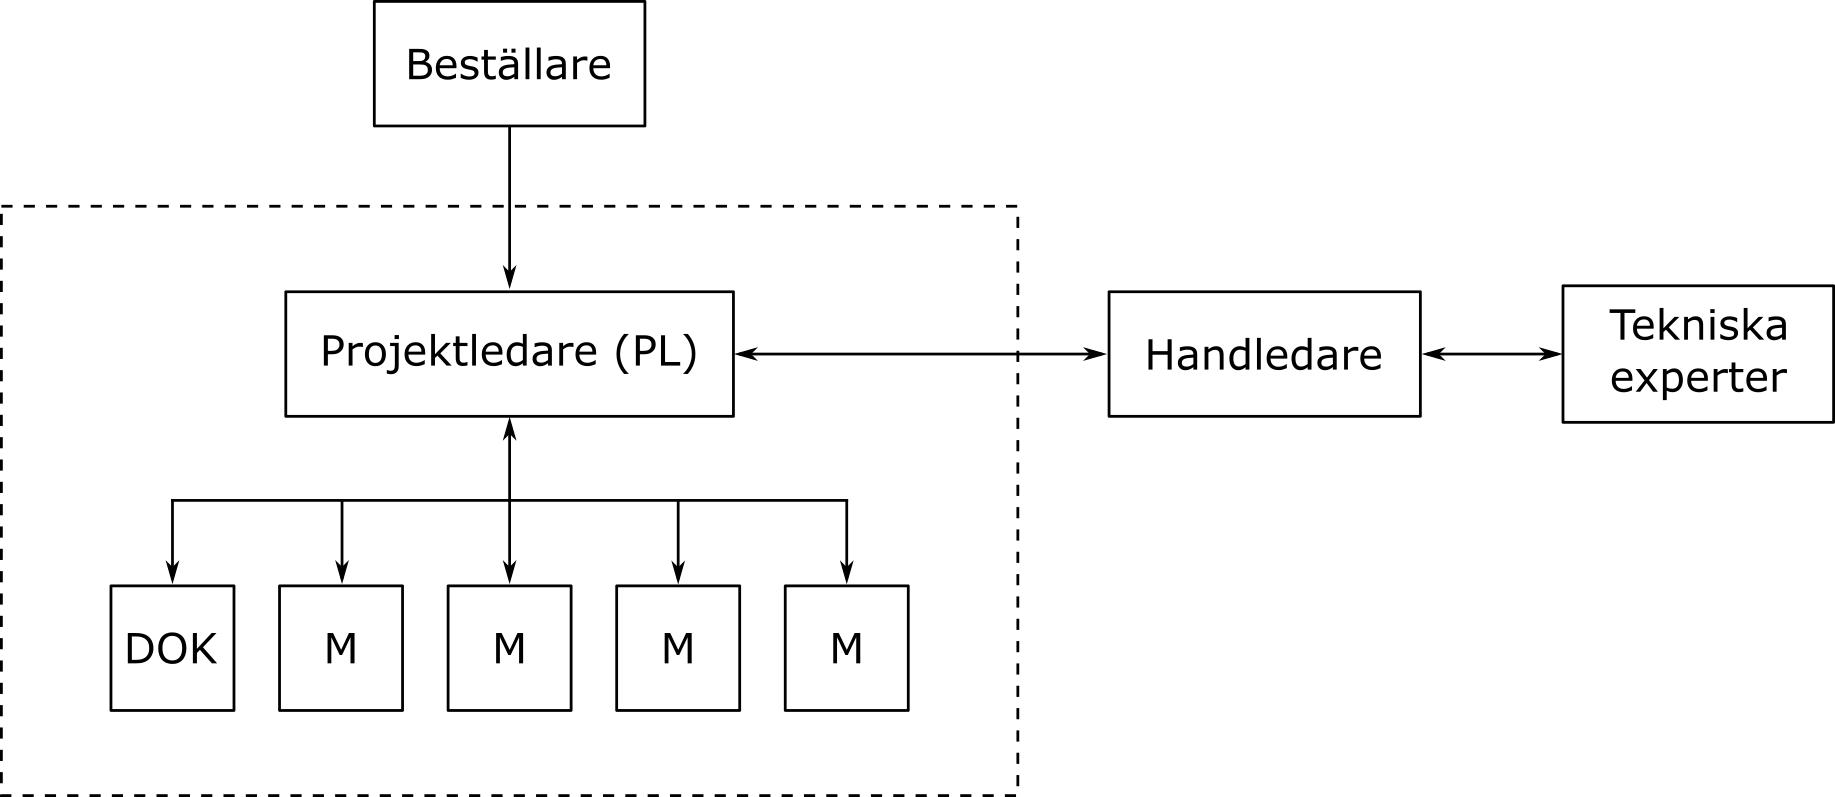
\includegraphics[scale=1]{organisation.png}
\caption{Översiktlig projektorganisation.}
\label{fig:org}
\end{figure}

\subsection{Villkor för samarbetet inom projektgruppen}
Följande punkter har beslutats gemensamt av projektgruppen och ska anses vara riktlinjer för hur samarbetet inom gruppen ska ske. Övriga frågor ska tas upp internt på gruppmöten.

\begin{itemize}
\item Deltagarna i gruppen ska gemensamt göra upp ordningsregler för gruppen om tider, närvaro, förberedelser, etc.
\item Alla deltagare i gruppen ska delta vid de tillfällen som gruppen kommit överens om.
\item Alla deltagare i gruppen ska komma väl förberedda till möten och dylikt, i den mån att det är nödvändigt för gruppens fortsatta arbete.
\item Alla deltagare i gruppen förväntas självständigt kommunicera med övriga gruppmedlemmar och arbetsgrupper för att underlätta sina egna och övrigas arbetsuppgifter.
\item Alla deltagare i gruppen ska ha en professionell inställning till arbetet som ska utföras.
\item Alla deltagare i gruppen kan ta upp interpersonella konflikter och frågor på möten för att säkerställa ett hälsosamt samarbete.
\item Problem med deltagare som inte bidrar till det gemensamma arbetet ska i första hand lösas internt, men kan vidarebefordras till kurspersonal om problemet kvarstår.
\item Alla deltagare i gruppen ska vara öppna för konstruktiv kritik.
\item Grupparbetet ska prioritera intresse framför resultat. En gruppmedlem ska inte vara tvingad att arbeta med någon visst område enbart för att vederbörande är den bäst lämpade för arbetet.
\item Vid schemalagda arbetstillfällen och projektmöten ska 'akademisk kvart' tillämpas.
\item Alla deltagare i gruppen har möjlighet att jobba hemifrån utefter eget schema efter samröre med berörda gruppmedlemmar.
\item Alla deltagare i gruppen ska vara kontaktbara under schemalagd arbetstid.
\end{itemize}

\subsection{Definition av arbetsinnehåll och ansvar}

\section{Dokumentplan}
Dokument ska i största möjliga mån följa tillgängliga LIPS-mallar. Dokumentansvarig är i fall där LIPS-mall saknas ansvarig för att skapa eller i övrigt godkänna dokumentmallar vid behov. Dokument ska lagras på sådant sätt att alla gruppmedlemmar (och enbart dessa) har tillgång till alla dokument över internet. Alla dokument ska skrivas på svenska, men teknisk dokumentation i källkod bör skrivas på engelska. 

Dokument ska revisionsnumreras på formatet \textit{\textless version\textgreater .\textless utgåva\textgreater}, där versionsnummer under 0 ska anses vara interna utkast, och version 1 är redo för leverans eller arkivering beroende på dokumenttyp. Att tilldela ett nytt versionsnummer innebär stora förändringar till dokumentets väsentliga innehåll. Utgåvenumret betecknar mindre förändringar som inte ändrar dokumentets väsentliga innehåll. Alla nya revisioner efter 1.0 av dokument som ska levereras till beställare måste göras i samröre med denne.

\section{Utvecklingsmetodik}

\section{Utbildningsplan}
\subsection{Egen utbildning}
Alla gruppmedlemmar ska genomföra en laboration i mätteknik, vilket innefattar att lära sig att använda en logikanalysator. Utöver detta förväntas alla gruppmedlemmar egenhändigt söka upp den kunskap och utbildning som krävs för att utföra sina tilldelade arbetsuppgifter.

\section{Rapporteringsplan}

\section{Mötesplan}
För alla möten gäller att projektledaren kallar till möte efter samråd om tillfälle med övriga gruppmedlemmar. Mötesprotokoll ska föras utefter LIPS-mallen. Alla gruppmedlemmar kan föra protokoll, men mötesprotokoll måste godkännas av projektledare eller dokumentansvarig.

Regelbundna projektmöten ska ske veckovis, företrädesvis i början av varje vecka. Vid dessa möten ska den gångna veckans arbete redovisas och utvärderas. Vidare ska en plan för grupparbetet fram tills nästa möte beslutas. Dessa möten ska hållas korta, helst under en timme per mötestillfälle. 

Utöver dessa projektmöten kan alla gruppmedlemmar föreslå möten vid behov. Dessa möten kan exempelvis handla om att fånga upp problem så tidigt som möjligt, eller göra en funktionalitets- eller kodgenomgång.

\section{Resursplan}
Här beskrivs vilka personer som jobbar med projektet, samt deras uppgifter. Även ekonomi, och lokaler, samt vilken material som behövs kommer att behandlas i detta kapitel.

\subsection{Personer}
Projektmedlemmarna:
\begin{itemize}
	\item Felix Härnström, Projektledare
	\item Emil Norberg, Dokumentansvarig
	\item Hannes Haglund, Designansvarig mjukvara
	\item Daniel Månsson, Designansvarig hårdvara
	\item Silas Lenz, Testansvarig
	\item Jani Jokinen, Leveransansvarig
\end{itemize}
Hannes Haglund kommer att vara bortrest under sista veckan av projektet.
Schemalagd tid är prioriterat för arbete och samtliga deltagare är upptagna under andra kursers föreälsningar och moment.
Handledaren för projektet är änsålänge okänd, men under projektetsgång kommer vi kunna rådfråga honom när problem uppstår, samt diskutera våra lösningar. Projektgruppen kommer träffa handledaren mindre i början och mer i slutet av projektet.

\subsection{Materiel}
Beställaren förser den hård- och mjukvara som krävs för att genomföra projektet. Gruppen kan i samröre med beställare göra förfrågan om att införskaffa ytterligare materiel. 

Följande material behövs till Kartrobotten
\begin{itemize}
	\item 1st Raspberry Pi 3
	\item 2st ATmega1284
	\item 1st LIDAR-lite v2
	\item 1st LSM9DS0
	\item 4st Ultraljud sensorer
	\item 2st Switchar
	\item A/D omvandlare
	\item Dator
	\item Motor till roterande sensor på taket
	\item Robotgrund, med hjul och motorer
\end{itemize}

\subsection{Lokaler}
Gruppen har tillgång till minst en arbetsstation i laborationsytan MUXEN.

\subsection{Ekonomi}
Gruppen ska efter beslutspunkt 2 arbeta 160 timmar per person. Genomfört arbete ska redovisas veckovis till beställaren.

\section{Milstolpar och beslutspunkter}
\subsection{Milstolpar}
\subsection{Beslutspunkter}

\section{Aktiviteter}

\section{Tidplan}

\section{Förändringsplan}

\section{Kvalitetsplan}

\subsection{Granskningar}

\subsection{Testplan}

\section{Riskanalys}

\section{Prioriteringar}

\section{Projektavslut}

\begin{appendices}
\end{appendices}
\end{document}
